\section{Simple examples of ZKPs}
\justify
As you can imagine, this powerful concept has a wide range of applications, from authentication systems to secure blockchain transactions. But first, in the following examples, we will explore simple cases of Zero-Knowledge Proof to illustrate how this technique works in practice, and then, go into further details.\cite{chainalysis2024}

\subsection{Proof of Membership}
Another way to understand zero-knowledge proofs is through the example of a locked safe. \cite{CirculariseZKPExamples} Imagine you meet someone who says he is part of your group, but you are not sure if you can trust him. Your group has a locked safe, and only members know the secret code to open it. To test him, you put a secret message inside the safe.
\\
\textbf{Protocol:}
\begin{enumerate}
\raggedright
    \item The Verifier writes a secret message and places it in the locked safe.
    \item The Prover, who knows the code, opens the safe.
    \item The Prover returns the secret message to the Verifier.
    \item The Verifier is convinced that the Prover knows the code and can be trusted.
\end{enumerate}

\begin{figure}[h!]
\centering
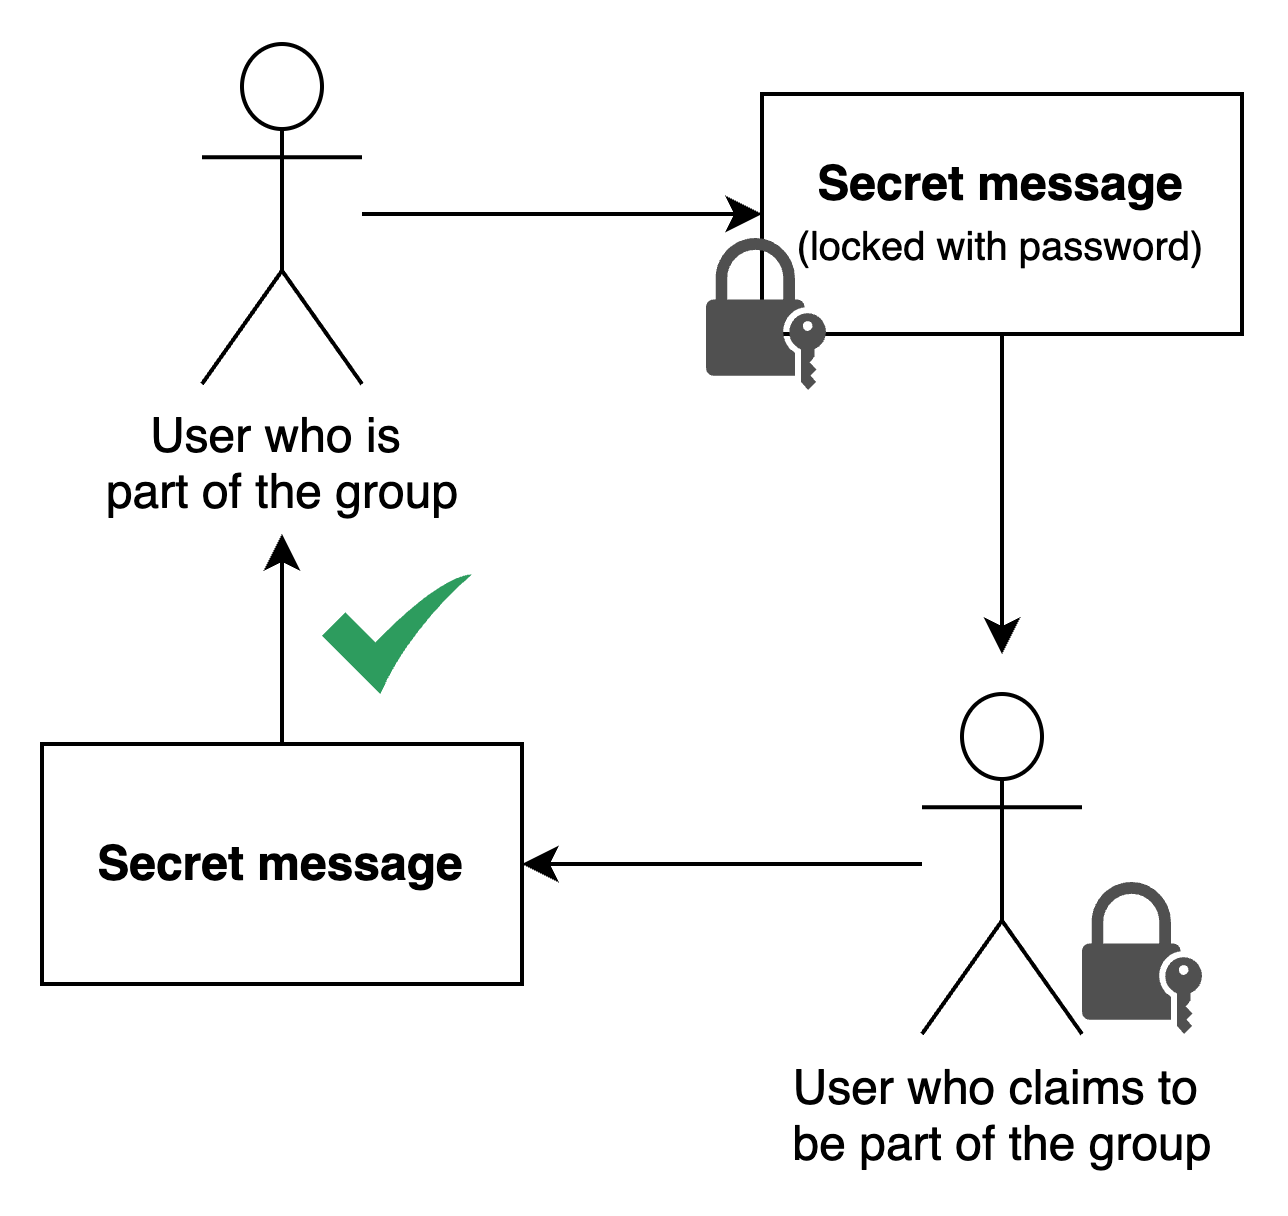
\includegraphics[scale=0.15]{Simple Examples/membership.png}
\caption{Proof of Membership flowchart.}
\end{figure}

If he can open the safe and return your message, it proves he knows the code without revealing the code itself. This is how interactive zero-knowledge proofs work: only those with the secret can prove their membership without giving away the secret itself.

\subsection{Salary verification}

Another way to understand zero-knowledge proofs is with a salary verification example.
\\
Imagine you and a colleague want to know if you are earning the same salary without revealing your exact salaries. You do not trust each other enough to share this information, and you are legally bound to keep your salaries private. Here's how you can find out using a zero-knowledge proof.
\\
\textbf{Protocol:}
\begin{enumerate}
    \item There are 4 locked boxes labeled with possible salaries interval: [1000-2000], [2000-3000], [3000-4000], and [4000 and more].
    \item You go into a private room. Since your salary is 2100, you take the key from the box labeled [2000-3000] and destroy the keys for the other boxes.
    \item Your colleague enters the room with 4 pieces of paper: 1 with a check and 3 with crosses. Since he earns 3300, he put the check in the box labeled [3000-4000] and crosses in the others.
    \item You return and open the box labeled 2000. Inside, you find a cross, so you know that your colleague does not earn the same salary as you.
    \item You close the box and put the cross on the table.
    \item Your colleague returns and sees you found a cross, so they know your salaries are different too.
\end{enumerate}
\begin{figure}[ht!]
\centering
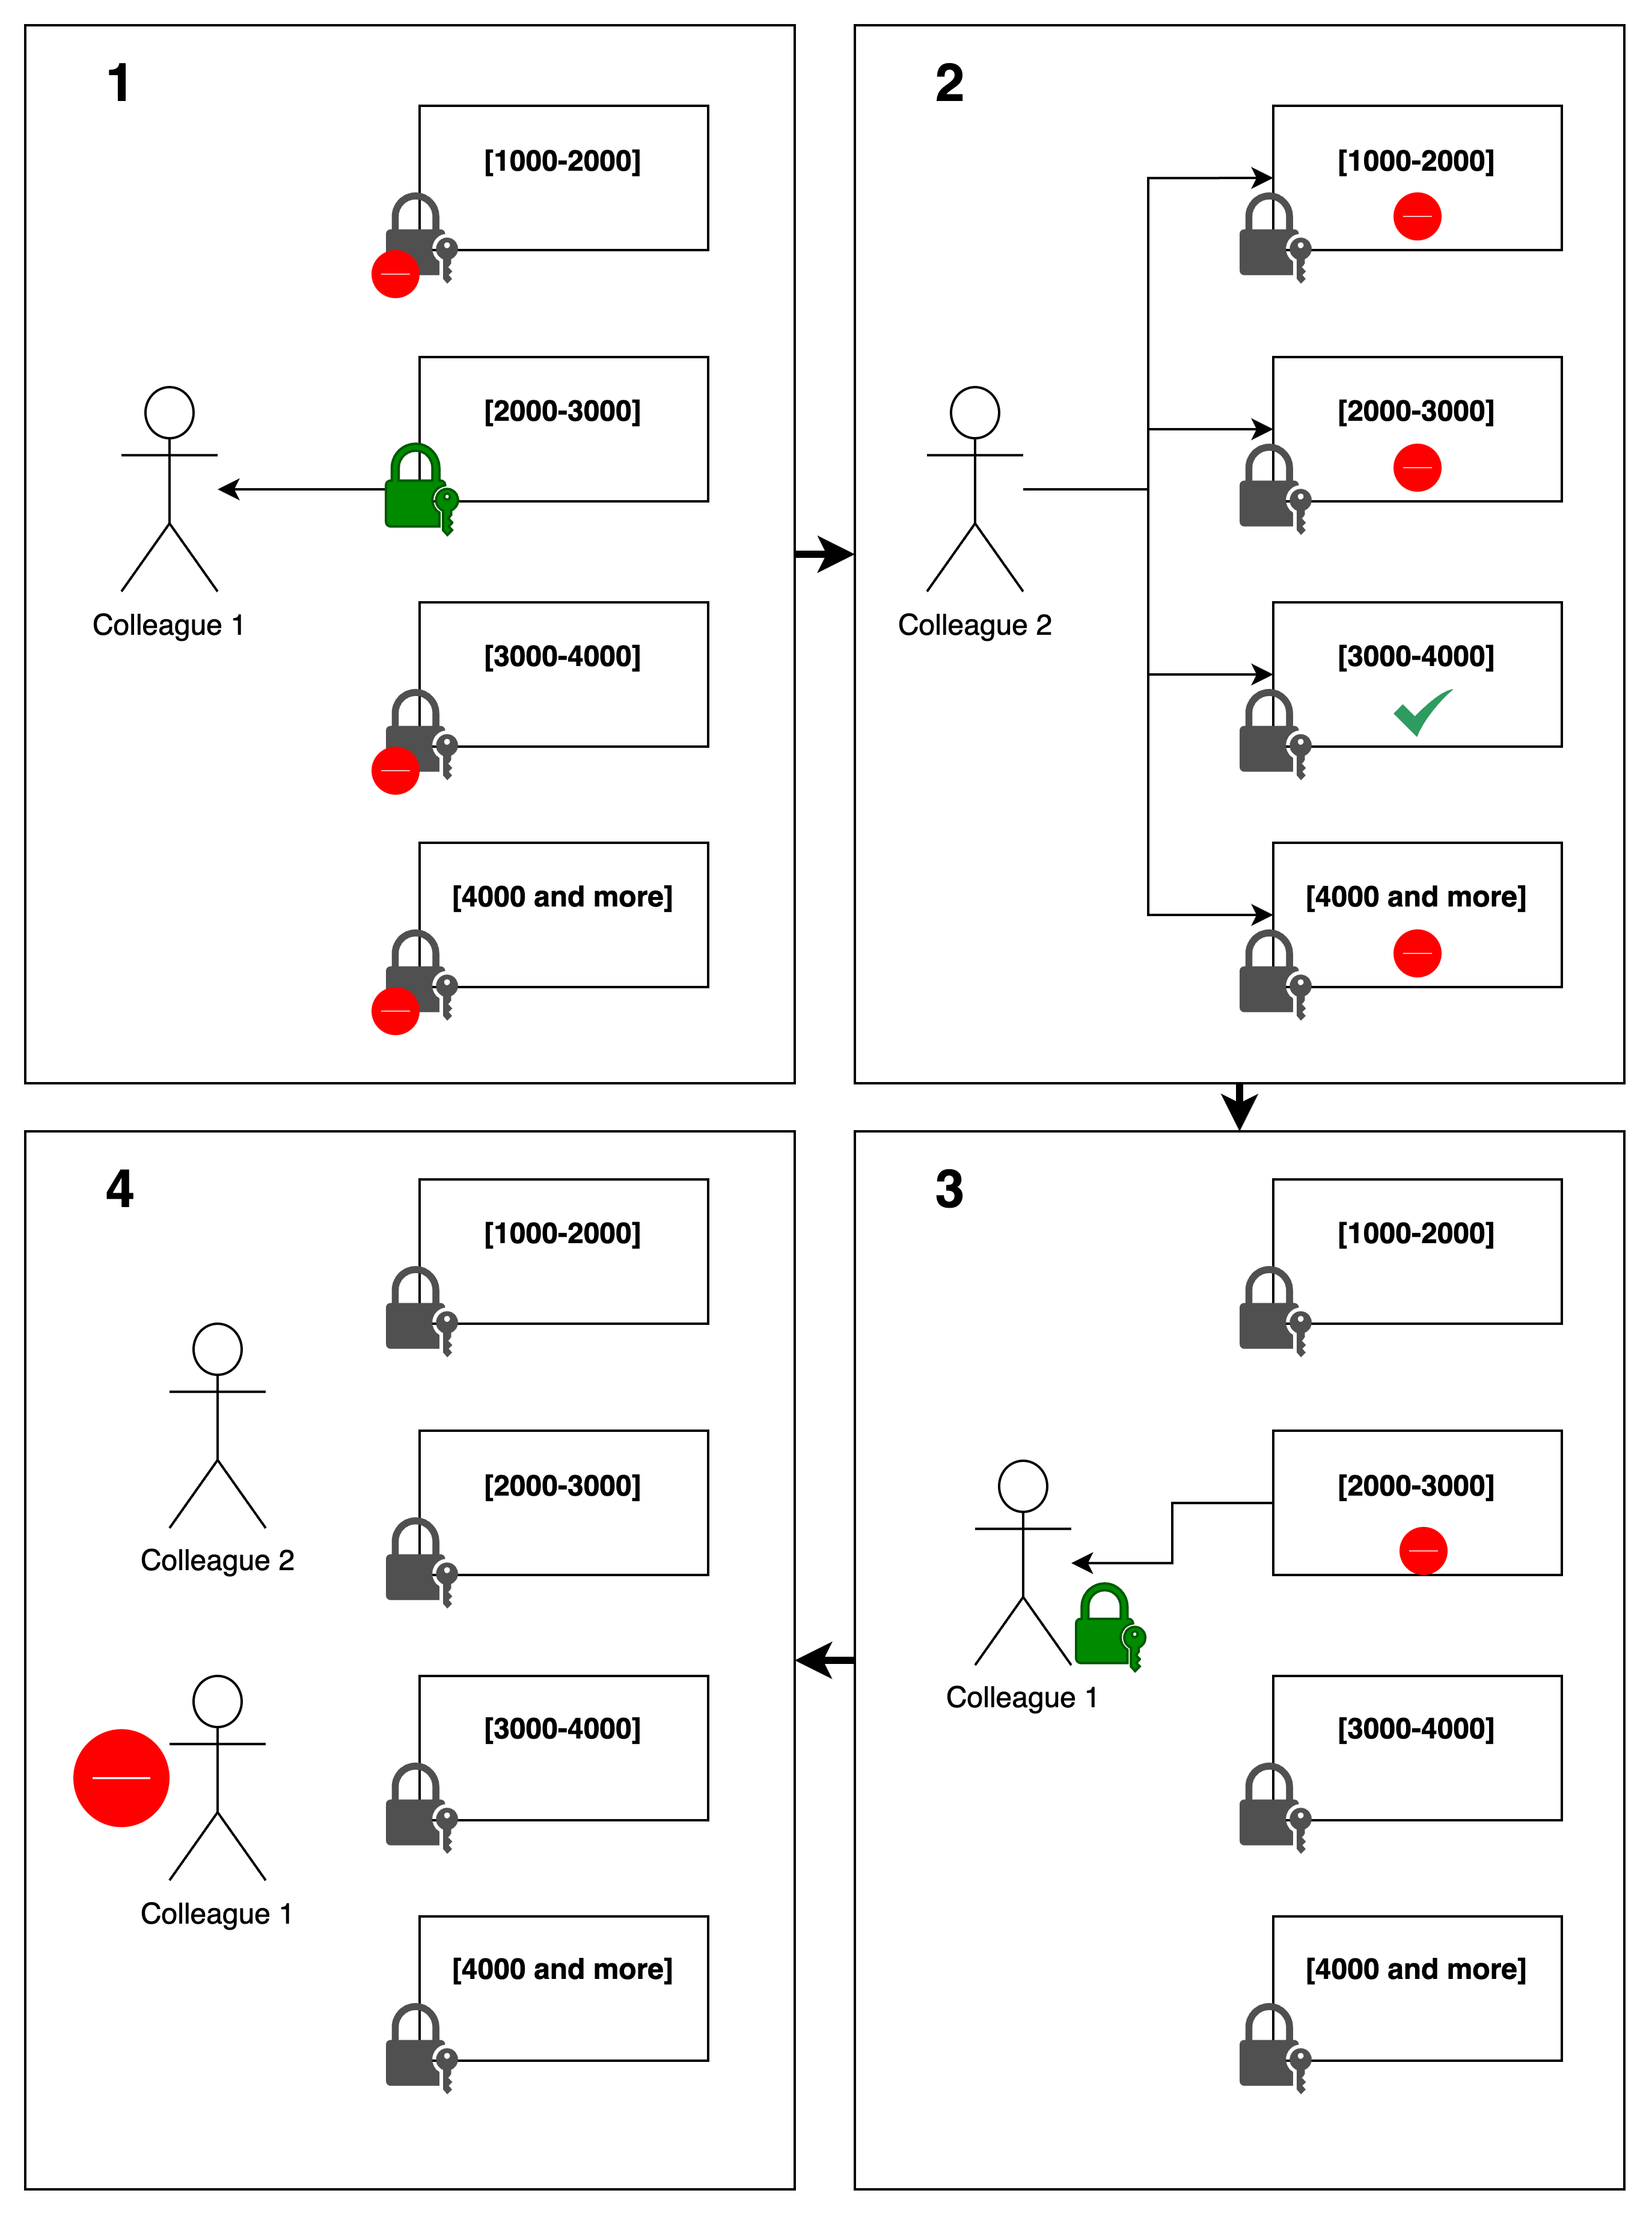
\includegraphics[scale=0.09]{Simple Examples/salary.png}
\caption{Salary verification flowchart.}
\end{figure}

If the paper had a check, you would both know your salaries are the same. But since you found a cross, you only learn that the salaries are different, without knowing the exact amount the other is earning.
\\
This example illustrates how zero-knowledge proofs can be used to verify information without revealing sensitive details.
